\documentclass[a4paper, 14pt, twocolumn]{article}

\usepackage{xeCJK}
\usepackage{ctex}
\usepackage{graphicx}
\usepackage{listings}
\usepackage{float}
\usepackage{caption}[font=small,labelfont=bf]
\usepackage{algorithm}  
\usepackage{algpseudocode}  
\usepackage{multirow}


\usepackage{amsmath,amsfonts,amsthm,amssymb}
\theoremstyle{definition}
\newtheorem{thm}{Theorem}
\newtheorem{exmp}{Example}
\newtheorem{defn}{Definition}
\newtheorem{lema}{Lemma}
\newtheorem{prop}{Proposition}
\newtheorem{coro}{Corollary}


\renewcommand{\baselinestretch}{1.25}
\renewcommand{\algorithmicrequire}{\textbf{Input:}}
\renewcommand{\algorithmicensure}{\textbf{Output:}}

\setlength{\textwidth}{162mm}
\setlength{\textheight}{190mm}
\setlength{\textheight}{231mm}
\setlength{\headheight}{-0.1cm}
\setlength{\topmargin}{-0.1cm}
\setlength{\oddsidemargin}{-0cm}
\setlength{\evensidemargin}{-0cm}


\setlength{\parskip}{1mm}
\setlength{\unitlength}{1mm}
\setlength{\parindent}{2em}

\lstset{
    basicstyle          =   \sffamily,          % 基本代码风格
    keywordstyle        =   \bfseries,          % 关键字风格
    commentstyle        =   \rmfamily\itshape,  % 注释的风格,斜体
    stringstyle         =   \ttfamily,  % 字符串风格
    flexiblecolumns,                % 别问为什么,加上这个
%    numbers             =   right,   % 行号的位置在左边
    showspaces          =   false,  % 是否显示空格,显示了有点乱,所以不现实了
    numberstyle         =   \zihao{-5}\ttfamily,    % 行号的样式,小五号,tt等宽字体
    showstringspaces    =   false,
    captionpos          =   t,      % 这段代码的名字所呈现的位置,t指的是top上面
    frame               =   lrtb,   % 显示边框
}

\lstdefinestyle{Python}{
    language        =   Python, 
    basicstyle      =   \zihao{-5}\ttfamily,
    numberstyle     =   \zihao{-5}\ttfamily,
    keywordstyle    =   \color{blue},
    keywordstyle    =   [1] \color{teal},
    stringstyle     =   \color{magenta},
    commentstyle    =   \color{red}\ttfamily,
    breaklines      =   true,   
    columns         =   fixed,  
    basewidth       =   0.5em,
}


\title{PageRank算法和MapReduce框架}
\author{王家蔚}
\begin{document}	
\maketitle


\begin{abstract}
对于一个特定的查询,搜索结果的排名取决于两方面的信息,第一个是关键字与网页的相关性,第二个是网页本身的质量,本文着重于第二点,也就是介绍一种被证明行之有效的评估网页质量的办法及其并行计算策略。

如今的全球搜索引擎巨头Google,最早的革命性发明是一款名为PageRank的算法,它是用来衡量网页本身的重要性的,核心思想并不复杂,发明人将互整个互联网想象成一张相互关联的有向图,如果图里的每个结点如果一个网页被其他很多网页链接,那么就说明该网页很重要,是受到普遍认可的,那么它的排名就要高。\cite{SearchEngine}

算法具体的实现方法涉及到图论和线性代数,为了更快地进行稀疏矩阵的运算,Google还专门开发了并行计算工具MapReduce,本文旨在先清晰地说明其中的技术细节,然后用Python和C++程序重现这一经典算法,并且针对常见关键字进行测试。
\end{abstract}

\section{引言}
在上世纪末,互联网上的网页数量快速增多,传统的搜索引擎,例如AltaVista和Yahoo,疲于应付新的趋势,主要原因是他们的算法是根据关键词分类所收录网站的。\cite{Wave}但是对于应对大规模的查询业务,很少有学术研究涉及到相关工程领域。Google的这项技术在1998年前后使得搜索引擎的结果在相关性方面取得了质的飞跃,具体表现在改善了网页的排序上,同时也完美地支持了高并发状态,从而一举超过Yahoo成为行业领头羊。

互联网发明最初是为了更高效地传递学术信息,在发展过程中,商业信息逐渐变成了主流内容,商业网站的占比从1993年的1.5\%上升到1997年的超过60\% \cite{Web},但是学术内容和商业网站之间存在着明显的差别,商业网站可以通过程序自动创建大量指向特定网站的链接,使自己的网站排名提高以谋求利润。所以Google在满足学术研究需求的同时,兼顾商业运营,以一种截然不同的方式对商业网站排名。Google这个项目的最终目的是要建立起一个覆盖全球互联网的网页索引大全。
\section{文献综述}
PageRank这方面的文章和工作主要由谢尔盖$\cdot$布林和拉里$\cdot$佩奇为代表的谷歌公司工程师完成,引用来介绍这个算法的文章大多也由他们亲自撰写。

不过在他们之前,已经有了一些开发文本链接结构系统的工作,Pitkow已经尝试用网页链接分析万维网的环境\cite{Ecology},Spertus把拥有链接结构的系统用在了数据挖掘上\cite{mining},此外还有人从不同的角度出发,也在对网页质量进行评估\cite{library}。当时的搜索引擎巨头也是把链接结构当作重要指标来优化搜索结果,但是这些项目都是简单地以链接数目作为评判标准,忽略了不同网站的链接权重并不相等这一事实,后面会仔细介绍这点。
\section{研究方法}
\subsection{PageRank算法}
\subsubsection{核心思想}
我们可以假设现在所有的网页都是图上的节点,网页之间的链接是有向边,每个节点都有一定数量的入链接(inedges)和出链接(outedges),被链接数大的网页很大概率就是更加重要的网页。\cite{CitationRanking}

此外也要考虑到这样一种情况,某一个网页被连接数不多,但都是被比较重要的网页所链接,比如如下图所示有一个网页C,只有两个网页A和B链接了它,但是这个网页B相当重要,收到了1000个其他网页的链接,那么网页A的重要性就不是单纯一个被链接数量能够描述的。
\begin{figure}[H]
\centering
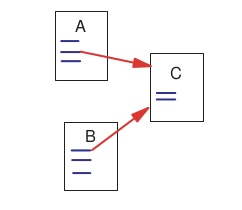
\includegraphics[width=2in]{figure/filelink.jpg}
\caption{特殊文件链接情况}
\end{figure}
为了通过链接更加合理地度量网页的重要性从而解决这个问题,不同网页被赋予了不同的权重,换句话说,如果一个网页想要得到高的排名,那么链接它的网页排名也需要尽可能地高。

\subsubsection{随机浏览者假设}
首先我们假设有一个网页的浏览者,他随机点击网页上的一个链接,一直持续下去。但是有可能网页上的链接是循环往复的,所以按照假设,他会一直持续点击这些链接。事实上,并不会有人真的这样做,如果碰到循环的情况,真实世界的浏览者肯定会重新打开一个新的网页,而且每次用户不一定会一直点击到没有链接为止,每当打开一个新网页,浏览者的下一步行为都有可能是打开一个不被现在网页直接链接的随机网页\cite{Surfer}
\begin{figure}[H]
\centering
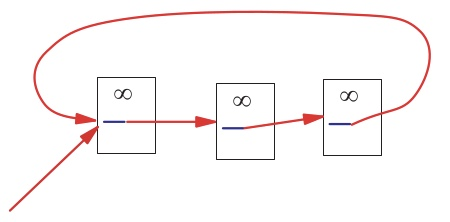
\includegraphics[width=3in]{figure/PageLoop.jpg}
\caption{循环的网页链接}
\end{figure}
为了在算法中模拟出在这个情况下的用户行为,我们需要一个$N$维向量$E$来存储随机浏览者转跳到不同网页的概率,其中的$N$是收录的网页数量。一般来说,我们继续假定每个网页被点击的概率都是相等的,当然这是一个可以个性化的参数,而且直接影响到收敛速度。关于向量$E$的进一步说明,我把它放在了第四部分。这小节假设的情况是为了给接下来介绍计算得分的方法作铺垫。
\subsubsection{计算方法}
假设网页A被n个网页所链接,这些网页分别记为$T_1,T_2,\cdots,T_n$,令$C(T_i)$表示网页$T_i$的出链接数量,接着我们还需要一个衰减系数$d \in (0,1)$,这是为了让每个网页在开始迭代的时候都有一定的保底分数。那么网页A的重要性得分可以按照以下的公式得出
\begin{equation*}
PR(A) = (1-d) + d(\frac{PR(T_1)}{C(T_1)} + ... + \frac{PR(T_n)}{C(T_n)})
\end{equation*}
这里的$d$一般取0.85。我们可以借助下图来直观的理解不同链接权重的含义
\begin{figure}[H]
\centering
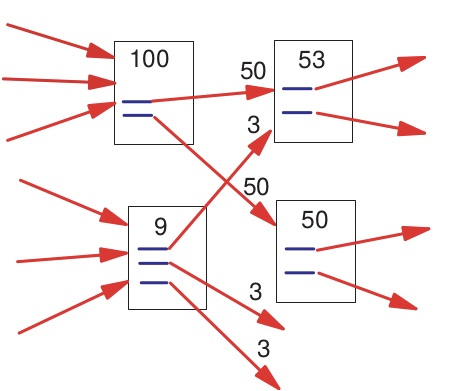
\includegraphics[width=3in]{figure/PageWeight.jpg}
\caption{带权重的链接}
\end{figure}
之后为了求出网页A的得分,我们要解决的问题是获取$T_1,T_2,\cdots,T_n$得分,这些网页又会有链接到它的其他网页。如果不存在循环链接的情况,那么从最底层的网页分数依次网上累加;如果存在如随机浏览者假设中循环链接的情况,那么就不存在最底层的网页,无法自底向上加出总分。为了解决这个问题,PageRank算法把问题转变成了一个二维矩阵相乘的问题,并用迭代的方法最终解决了它。

具体来看这个迭代的过程,首先我们把所有网页都给予从$1$到$N$的唯一编号,把它们的对应的最终得分记录在$N$维向量
\begin{equation*}
B=[b_1,b_2,\cdots,b_N]^T
\end{equation*}
中,然后把链接结构用如下的矩阵
\[A=
\begin{bmatrix}
a_{11} & a_{12} & \cdots & a_{1N} \\
\vdots &        &        & \vdots \\
a_{m1} & a_{m2} & \cdots & a_{mN} \\
\vdots &        &        & \vdots \\
a_{N1} & a_{N2} & \cdots & a_{NN} \\
\end{bmatrix}
\]
记录下来,其中的$a_{mn}$表示第m个网页指向第n个网页的链接数,迭代起点设置为
\begin{equation*}
B_0=[\frac{1}{N},\frac{1}{N},\cdots,\frac{1}{N}]^T
\end{equation*}
迭代公式设置为
\begin{equation*}
B_{n+1}=AB_n+(||AB_n||_1-||B_n||_1)E
\end{equation*}
完整过程我用伪代码的形式给出
\begin{algorithm}[htb]  
\caption{PageRank伪代码}  
\label{alg:PR}  
    \begin{algorithmic}[1]  
     \Require  
          迭代收敛误差的容忍极限$\epsilon$
          
          存储网页链接结构的矩阵$A$
          
          存储网页初始得分的向量$B_0$
          
          浏览者跳转概率向量$E$
     \Ensure  
          存储网页最终得分的向量$B$
     \Function {PageRank}{$A,B_0,E,\epsilon$}
     \State $d=||AB_0||_1-||B_0||_1$
     \State $B_1=AB_0+dE$
     \State $\delta = ||B_1-B_0||_1$
     \While{$\delta > \epsilon$}
     \State $B_{i+1} = AB_{i}$
	 \State $d=||B_{i+1}||_1-||B_{i}||_1$     
	 \State $B_{i+1}=B_{i+1}+dE$
	 \State $\delta = ||B_{i+1}-B_i||_1$
     \EndWhile
     \State $B=B_{i+1}$
     \State \Return{$B$} 
     \EndFunction     
     \end{algorithmic}  
\end{algorithm}  

简明扼要说明以下思路,首先要明确的输入和输出,既然是企图用迭代操作获取收敛值,那么就不能期望得到精确解,必须要设置一个误差限$\epsilon$,其他的输入输出量前面都已经提到,这里不再赘述。之后先在循环外进行一次迭代,把$\delta$初始化,之后进入while循环,特别注意为了简化计算复杂度,向量间的距离用1范数给出。最后当$\delta<\epsilon$时,就进行输出。
\subsubsection{收敛证明}
取$e$为所有分量都为1的列向量,定义矩阵
\begin{equation*}
M=\alpha E+\frac{1-\alpha}{N}ee^T
\end{equation*}
那么上述的迭代过程就是$B_n=MB_{n-1}$​, 于是该问题就转为了一个Markov过程了。马尔科夫链的收敛条件如下\cite{Convergence}
\begin{itemize}
\item[•]M为随机矩阵
\item[•]M是不可约的
\item[•]M是非周期的
\end{itemize}
以上条件均满足,所以pagerank是收敛的,且与初始值无关,即无论$B_0$取值如何,都不会影响最后各个网页的得分情况。
\subsubsection{部分源代码}
\lstinputlisting[
    style       =   Python,
    caption     =   {\bf 生成评分的函数模块},
    label       =   {PR}
    ]{pr.h}
\subsection{MapReduce框架}
\subsubsection{核心思想}
从前面的算法可以看出,为了给新收录的网页评分,PageRank算法反复做大规模的矩阵运算,而且计算量每次都会增加,很紧迫的需求就是切分矩阵实现并行计算。针对挑战,Google给出的解决方案是一个叫做MapReduce的程序,它的核心设计思想是分治算法。\cite{Math}

将一个大任务拆分成若干个子任务,并且完成子任务的计算,这个过程叫做\textit{Map},将中间结果合并成最终要的结果,这个过程叫做\textit{Reduce}。还有很多更加具体的问题需要考虑,比如平均分配负载,分布式存储数据,错误容忍。\cite{MapReduce}

MapReduce框架给出的是一个并行计算的通用解决方案,文件首先要输入(input)程序,然后进行切分(split),把每一个片段分配(map)到不同的工作站(worker)中,计算的结果分布的存储在本地,之后由远端的工作站(worker)逐个读取结果并且重新排序(shuffle),最后一步才是合并(reduce)输出最终的文件。具体的过程见下图
\begin{figure}[H]
\centering
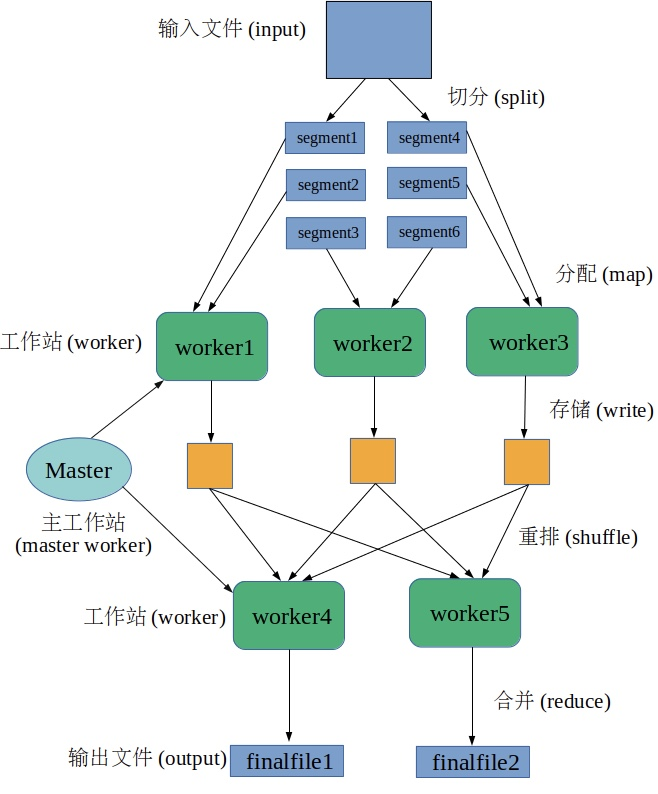
\includegraphics[width=3in]{figure/MapReduce.jpg}
\caption{MapReduce架构}
\end{figure}
此外还有一个需要强调的部分是,过程中还会产生一个主工作站(master worker),这个和其他工作站等级是一样的,只不过会做一些特殊事情,它会作为用户的代理来协调整个过程,用户就可以做其他事情。主工作站会让一个工作站去拿1号数据,另一个工作站负责拿2号数据等等,这就是分配数据的过程。抽象地说,主工作站是将map任务产的中间数据位置传送到reduce任务的管道,所以主工作站保存了map任务完成后产生的若干中间文件的位置信息包含大小,当然,map任务结束的时候会更新位置和大小信息。这个信息会被逐步的推送到正在处理reduce任务的工作站。
\subsubsection{矩阵运算}
由于PageRank算法涉及到大规模矩阵并行计算,所以这里特别说明一下MapReduce在处理矩阵乘法上的应用。我们先讲理论抽象,假设我们有规模为$m \times n$的矩阵$A$和规模为$n \times p$的矩阵$B$,两者相乘得到矩阵$C$.就以$a_{11}$为例,它将会在$c_{11},c_{12},\cdots,c_{1p}$的计算中使用。也就是说,在Map阶段,当我们从切分完毕的文件中取出一行记录时,如果该记录是$A$的元素,则需要存储成$p$个<$key$, $value$>对,并且这$p$个$key$互不相同;如果该记录是$B$的元素,则需要存储成$m$个<$key$, $value$>对,同样的,$m$个$key$也应互不相同;但同时,用于存放计算$c_{ij}$的$a_{i1},a_{i2},\cdots,a_{in}$和$b_{1j}、b_{2j},\cdots, b_{nj}$的<$key$, $value$>对的$key$应该都是相同的,这样才能被传递到同一个Reduce中。

举个例子,我们有规模为$3\times2$的矩阵$A$和规模为$2\times4$的矩阵$B$
\[C=AB=
\begin{bmatrix}
5 & 3 \\
10 & 2\\
1 & 1\\
\end{bmatrix} \times
\begin{bmatrix}
3 & 0 & 7 & 11\\
9 & 2 & 6 & 8\\
\end{bmatrix}
\]
在计算的时候,我们需要将矩阵$A$转换成下面这张键值表

\begin{tabular}{|l|l||l|l||l|l|}
\hline
key & value & key & value & key & value\\
\hline
1,1 & a,1,5 & 2,1 & a,1,10 & 3,1 & a,1,1\\
\hline
1,1 & a,2,3 & 2,1 & a,2,2 & 3,1 & a,2,1\\
\hline
1,2 & a,1,5 & 2,2 & a,1,10 & 3,2 & a,1,1\\
\hline
1,2 & a,2,3 & 2,2 & a,2,2 & 3,2 & a,2,1\\
\hline
1,3 & a,1,5 & 2,3 & a,1,10 & 3,3 & a,1,1\\
\hline
1,3 & a,2,3 & 2,3 & a,2,2 & 3,3 & a,2,1\\
\hline
1,4 & a,1,5 & 2,4 & a,1,10 & 3,4 & a,1,1\\
\hline
1,4 & a,2,3 & 2,4 & a,2,2 & 3,4 & a,2,1\\
\hline
\end{tabular}

这里的key是指这个数据用来计算矩阵$C$中哪个位置的值,比如第一行第一列这个位置对应$key=(1,1)$,计算过程涉及到矩阵$A$中的两个值,所以上表中同样的$key$也只对应两个$value$。$value$第一部分表示它属于哪个矩阵,第二部分表示它是原矩阵这一行/列第几个元素,只有对应的元素才能相乘,第三部分才是用来计算的数值,其余部分都是为了用来定位的。同样的办法可以得到矩阵$B$的键值表,如下所示

\begin{tabular}{|l|l||l|l||l|l|}
\hline
key & value & key & value & key & value\\
\hline
1,1 & b,1,3 & 2,1 & b,1,3 & 3,1 & b,1,3\\
\hline
1,1 & b,2,9 & 2,1 & b,2,9 & 3,1 & b,2,9\\
\hline
1,2 & b,1,0 & 2,2 & b,1,0 & 3,2 & b,1,0\\
\hline
1,2 & b,2,2 & 2,2 & b,2,2 & 3,2 & b,2,2\\
\hline
1,3 & b,1,7 & 2,3 & b,1,7 & 3,3 & b,1,7\\
\hline
1,3 & b,2,6 & 2,3 & b,2,6 & 3,3 & b,2,6\\
\hline
1,4 & b,1,11 & 2,4 & b,1,11 & 3,4 & b,1,11\\
\hline
1,4 & b,2,8 & 2,4 & b,2,8 & 3,4 & b,2,8\\
\hline
\end{tabular}
后面重排(shuffle)这步将分布式存储的数据按照$key$值进行归类

\begin{tabular}{|l|l|l||l|l|l|}
\hline
key & \multicolumn{2}{|c||}{values} & key & \multicolumn{2}{|c|}{values}\\
\hline
\multirow{2}*{1,1} & a,1,5 & b,1,3 & \multirow{2}*{1,2} & a,1,5 & b,1,0\\  \cline{2-3} \cline{5-6}
                   & a,2,3 & b,2,9 &                    & a,2,3 & b,2,9 \\ \hline

\multirow{2}*{1,3} & a,1,5 & b,1,7 & \multirow{2}*{1,4} & a,1,5 & b,1,11\\  \cline{2-3} \cline{5-6}
                   & a,2,3 & b,2,6 &                    & a,2,3 & b,2,8 \\ \hline

\multirow{2}*{2,1} & a,1,10 & b,1,3 & \multirow{2}*{2,2} & a,1,10& b,1,0\\  \cline{2-3} \cline{5-6}
                   & a,2,2  & b,2,9 &                    & a,2,2 & b,2,2 \\ \hline
                   
\multirow{2}*{2,3} & a,1,10 & b,1,7 & \multirow{2}*{2,4} & a,1,10& b,1,11\\  \cline{2-3} \cline{5-6}
                   & a,2,2  & b,2,6 &                    & a,2,2 & b,2,8 \\ \hline
                   
\multirow{2}*{3,1} & a,1,1  & b,1,3 & \multirow{2}*{3,2} & a,1,1 & b,1,0\\  \cline{2-3} \cline{5-6}
                   & a,2,1  & b,2,9 &                    & a,2,1 & b,2,2 \\ \hline                   
                   
\multirow{2}*{3,3} & a,1,1  & b,1,7 & \multirow{2}*{3,4} & a,1,1 & b,1,11\\  \cline{2-3} \cline{5-6}
                   & a,2,1  & b,2,6 &                    & a,2,1 & b,2,8 \\ \hline                       
\end{tabular}
最后一步是归并(reduce),依次对每一个$key$进行加总输出结果,这里就不列表进行展示了。
\subsubsection{部分源代码}
\lstinputlisting[
    style       =   Python,
    caption     =   {\bf Map过程模块},
    label       =   {PR}
    ]{mr.cpp}
\section{讨论}
PageRank算法为了解决循环链接的问题,$3.1.2$节引入了一个描述转跳概率的矩阵$E$,之前我们假设所有网页被转跳到的概率是一模一样的,实际上数值是被重新设置过的。在测试中发现,一些写有著作权,免责申明的网页被广泛链接,还有邮件服务器等没有实际内容的网页评分也很高。解决方案是只给各大网站的根目录给予一定的概率分布,另外对用户设置的家网页更高的概率。
\section{结论}
个人认为数学软件的最大作用,是根据你的想法,以最快速度做出一个模型,用来检验结果的有效性。使用者不需要重复造轮子,Matlab已经将绝大多数现在证明可行的办法,就拿课堂上和我作业里的例子来说,比如多层卷积神经网络和KDTree,线性回归等都已经完全封装在一个函数里,任何人只要理解了算法的原理,读一下自带文档的接口参数,就可以迅速得到想要的结果。完善友善的内置文档,让使用者不需要到处寻找技术博客查询某个特定功能的函数,大大提高了。

Matlab以接近自然语言的语法和丰富的扩展包为特点,配合上高效的矩阵计算,能解决大多数数学研究设计到的编程需求。控制系统设计与分析、金融工业建模和仿真模拟等领域都是它极度擅长的。高度封装性优点在于只要看文档明确输入输出的格式,完全不需要花费额外的时间去调试中间繁琐的实现过程,不仅如此,像Matlab这样成熟的商业软件在结果的正确性上也完全可以信任。总而言之,可以让数学研究者更多地专注于数学本身,尽可能少地与编程技巧较劲。

Matlab这样大型的商业软件的优点很明显,局限性也不小。首先它的解释器就已经超过了500M,如果要加上一些常用的扩展包,起码需要10G的存储空间,此外运行效率比较低,所以几乎只能将.m程序放在个人计算机上运行,不能放在一些小型的嵌入式系统上。由于不是开源的软件,所以也不能才剪掉某个特定程序不需要的部分,更不能做一些底层的优化。此外,对于软件工程师来说,长时间使用可能会导致变成水平下降;同样也不适合计算机编程领域的初学者,因为它几乎没有需要进行硬件操作的地方,就连并行的实现也轻而易举,gpu工具箱是把整个cuda打包了。

综上,Matlab语法简单,文档易懂,封装性好,扩展包多,所以是应用数学建模领域和学术研究的一个良好测试工具,相比于开源的Octave在运行稳定性上有明显的优势。但是运行效率上存在劣势,在大型商业项目的开发上,肯定无法代替编译型语言。
\begin{thebibliography}{99}
	\bibliographystyle{unsrt}
	\bibitem{SearchEngine}The Anatomy of a Large-Scale Hypertextual Web Search Engine, Sergey Brin and Lawrence Page
	\bibitem{Wave} On Top of Tides,Jun Wu
	\bibitem{Web}Web Growth Summary, Matthew Gray
	\bibitem{Ecology}Characterizing World Wide Web Ecologies, James E. Pitkow
	\bibitem{mining}Parasite: Mining structural information on the web, Ellen Spertus
	\bibitem{library}Evaluating quality on the net, Hope N. Tillman
	\bibitem{CitationRanking}The PageRank Citation Ranking: Bringing Order to the Web, Lawrence Page, Sergey Brin, Rajeev Motwani, Terry Winograd
	\bibitem{Surfer}PageRank and The Random Surfer Model, Prasad Chebolu and Páll Melsted
	\bibitem{Convergence}Convergence of Markov Chains in Information Divergence, Peter Harremoës and Klaus Kähler Holst 
	\bibitem{Math} Beauty of Mathematics, Jun Wu
	\bibitem{MapReduce}MapReduce: Simplified Data Processing on Large Clusters, Jeffrey Dean and Sanjay Ghemawat
\end{thebibliography}



\end{document}
